	%====================================================================================================
	% ?????
	%====================================================================================================
	% TCC
	%----------------------------------------------------------------------------------------------------
	% Autor				: Jasane Schio
	% Orientador		: Gedson Faria
	% Co-Orientador		: Angelo Darcy
	% Instituição 		: UFMS - Universidade Federal do Mato Grosso do Sul
	% Departamento		: CPCX - Sistema de Informação
	%----------------------------------------------------------------------------------------------------
	% Data de criação	: 01 de Outubro de 2015
	%====================================================================================================
	%descrever problemas e as solucoes encontradas
	\definecolor{dkgreen}{rgb}{0,0.6,0}
	\definecolor{gray}{rgb}{0.5,0.5,0.5}
	\definecolor{mauve}{rgb}{0.58,0,0.82}
	
	\lstset{frame=tb,
		language=C++,
		aboveskip=3mm,
		belowskip=3mm,
		showstringspaces=false,
		columns=flexible,
		basicstyle={\small\ttfamily},
		numbers=none,
		numberstyle=\tiny\color{gray},
		keywordstyle=\color{blue},
		commentstyle=\color{dkgreen},
		stringstyle=\color{mauve},
		breaklines=true,
		breakatwhitespace=true,
		tabsize=3
	}
	\chapter{Desenvolvimento} 
	\section{Considerações Iniciais}
	Neste capítulo descreve-se o sistema proposto, denominado SCIMM, as tecnologias utilizadas no projeto, a organização do projeto e suas classes, o fluxo do sistemas e cada uma das etapas do seu funcionamento.
	
	Para o desenvolvimento foi escolhida a biblioteca OpenCV por ser de código aberto\footnote{Modelo de desenvolvimento de {\it software}, no qual o código fonte é aberto e livre para modificações e adaptações}, multiplataforma, conter uma grande quantidade de métodos e algoritmos já implementados	e pelo seu rápido desempenho de máquina.
	
	A linguagem escolhida para o desenvolvimento foi o C++, pois é uma linguagem de programação compilada, o que torna sua execução mais rápida que as linguagem interpretadas, dando ao sistema uma performance em tempo satisfatório. 
			
	Todo o projeto foi desenvolvido em sistema operacional Ubuntu e utilizou-se a ferramenta {\it Github} como repositório {\it online} para o controle de versão do projeto. A escolha desse repositório se deve ao fato da plataforma conter um grande número de projetos de código aberto, e uma vez que este trabalho tem como finalidade principal beneficiar as equipe de times de futebol de robôs, deixar seu código aberto permite que melhorias possam ser adicionadas além de soluções para possíveis erros.
			
\section{Tecnologias Usadas}
Para realização deste trabalho,  utilizou-se a biblioteca de processamentos de imagens OpenCV. O trabalho foi elaborado na linguagem C++, com uso do {\it framework} Qt para a composição da interface gráfica.
 
\begin{description}
	\item[OpenCV] foi lançado em 1999 pela Intel\cite{Culjak:2012}, com objetivo de ser otimizada, portável e com um grande número de funções, se tornou uma ferramenta que possui mais de 2500 algoritmos e 40 mil pessoas em seu grupo de usuários\cite{Culjak:2012}. Já possui interface para as linguagens C++, C, Python e Java, além de suporte para as principais plataformas como Windows, Linux, Mac OS, iOS e Android. A biblioteca pode ser utilizada para manipular tanto imagens em tempo real, quanto vídeos e imagens estáticas.
	
	\item[Qt] é um {\it framework} de desenvolvimento de aplicações multiplataforma. Entre suas funcionalidades está a possibilidade de criar interfaces gráficas diretamente em C++ usando seu módulo{\it  Widgets}.
	
	\item [C++] é uma linguagem de programação projetada por \citeonline{Stroustrup:1996} para fornecer eficiência e flexibilidade da linguagem C para programação de sistemas. A linguagem C++ evoluiu a partir de um projeto chamado C com Classes que foi realizado  entre 1979 e 1983. A linguagem foi oficialmente lancada em 1986.
\end{description}

\section{Descrição do Projeto}
\subsection{Organização do Projeto}
	 O projeto foi desenvolvido seguindo o paradigma de programação Orientada à Objetos, esse paradigma baseia-se na utilização de objetos individuais para criação de um sistema maior e complexo. A IDE usada para o desenvolvimento foi a QT Creator, esta separada o projeto em três pastas: {\it Headers}, {\it Sources} e {\it Forms} (Figura \ref{fig:OrganizacaoDoProjeto}). Na pasta {\it Headers} estão os arquivos de cabeçalho(.h), onde estão as declarações dos métodos e variáveis usados nas classes  executáveis. Na pasta {\it Sources} estão os arquivos fonte(.cpp), são nesses arquivos que os métodos declarados nos arquivos da pasta {\it Headers} são implementados. Na pasta {\it Forms} está o arquivo de interface gráfica(.ui) que é usado no projeto.
	 
	\begin{figure}[H]
		\centering
		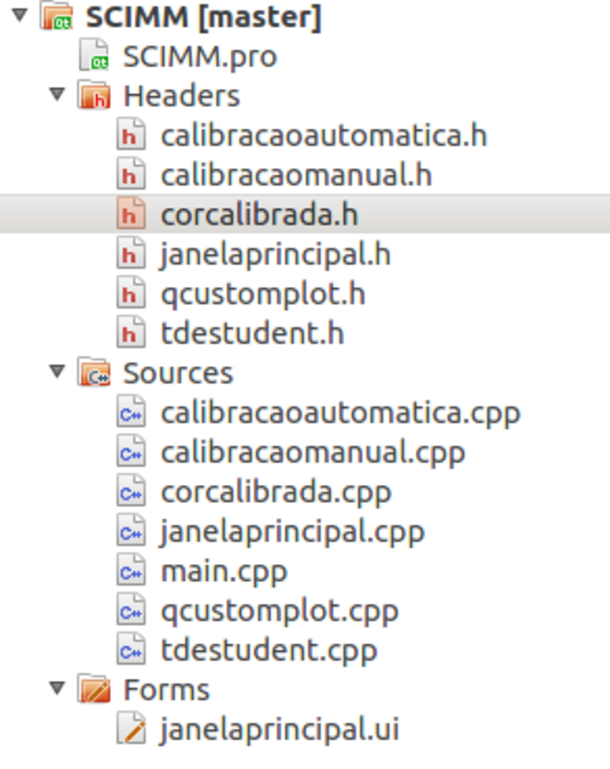
\includegraphics[width=0.2\textwidth]{organizacaoProjeto.pdf}
		\caption{Organização das pastas do projeto}
		\label{fig:OrganizacaoDoProjeto}
	\end{figure}
	%Com exceção do arquivo fonte main, cada arquivo de cabeçalho possui um arquivo fonte correspondente, formando assim um objeto, todo objeto é uma classe mas nem toda classe forma um objeto. As classes desenvolvidas no projeto são: calibracao, scimm\_cor e janelaprincipal.
%Para melhor entendimento da interação entre as classes a figura 3.2 trás o diagrama de classes do projeto.

\subsection{Apresentação das Classes}
\subsubsection{Classe main}
 Esta é o que se chama de \textit{ponto de entrada} em programação. \textit{Ponto de entrada} é onde o sistema operacional irá iniciar a execução do sistema desenvolvido. Esta classe possui somente o método \textit{main} e este instancia e inicia o objeto \textbf{JanelaPrincipal} que apresenta a interface gráfica para interação com o usuário.
 
\subsubsection{Classe JanelaPrincipal}
Nesta classe utiliza-se da implementação de objetos \textit{QWidget} e suas subclasses disponíveis pelo Qt, para a criação de uma interface gráfica que faz a interação com o usuário. Todos os métodos presentes nessa classe são para utilização gráfica, comportamento de botões e menu de seleção, e para a comunicação com a classe de calibração.	

\subsubsection{Classe Calibracao}
 Esta classe contém todos os métodos e variáveis usados no processo de calibração, é também dentro dessa classe que são feitas todos os tipos de manipulação em imagem.
 
Os métodos contidos na classe Calibração são:
	\begin{description}

\item Iniciar: Método utilizado para fazer referencia à \textbf{JanelaPrincipal}, devido a necessidade de comunicação com a interface que não seja por meio de retorno. Este método também inicializa a câmera, se esta estiver disponível.

\item ConfigurarCamera: Método utilizado para delimitar, um retângulo, ou seja, o espaço de trabalho dentro da imagem proveniente da câmera. Também é utilizada para ajuste de brilho e contraste para tornar mais nítido os contornos durante a detecção de objetos dentro do retângulo já delimitado.	
	
  \item ReconhecerFundoExtrairObjetos: Método no qual utiliza-se o algoritmo de subtração de fundo. Identifica-se, inicialmente, o campo e uma vez identificado, qualquer objeto colocado sobre o campo ficará em destaque pois não faziam parte do fundo inicial. Esse destaque é uma \textbf{máscara} sobre a imagem que é usada melhorar a precisão do algoritmo de detecção dos objetos.
  
 	\item DetectarObjetos: Método onde serão aplicados filtros de diminuição de ruido, detectadas as bordas existentes na imagem, detectados os objetos a partir das bordas contidas na imagem, o aumento da precisão do contorno dos objetos e diminuição do tamanho do objeto de acordo com a porcentagem de borda a ser eliminada. 

\item Calcular: Método utilizado para analisar cada pixel pertencente aos objetos detectados. O valor H do HSV é categorizado de acordo com as cores pre-definidas no sistema. % e adicionado a cor correspondente.
%O algoritmo de categorização:

\item Calibrar: Método utilizado para administrar a utilização dos métodos \textbf{DetectarObjetos} e \textbf{Calcular}. % para serem analisados os valores de cada pixel de cada objetos e estes classificados de acordo com as cores pré definidas pelo sistemas. Uma vez terminado o processo de calibração é exibida na tela para o usuário os objetos da cor que esta selecionada no menu de cores.		

	\item ObterPorcentagem: Método simples para devolver a porcentagem de um valor, ao ser informado o valor e a porcentagem escolhida.
		
		
	
		\end{description}	

\subsubsection{Classe SCIMM\_COR}
	Classe na qual se instancia cada cor que é reconhecida pelo sistema. Os objetos desse tipo armazenam os valores máximos e mínimos de H, S e V. 


\section{Detalhes de Implementação do Sistema SCIMM}

		 O sistema consiste na apresentação da \textbf{interface gráfica} objetiva. Possuindo seis botões, um menu de escolha e uma janela de exibição.
		 Na Figura \ref{fig:FlowCHart} pode ser observado o fluxo do sistema, que se constitui em cinco etapas com o mínimo de ação possível do usuário.
		
		\begin{figure}[H]
			\centering
			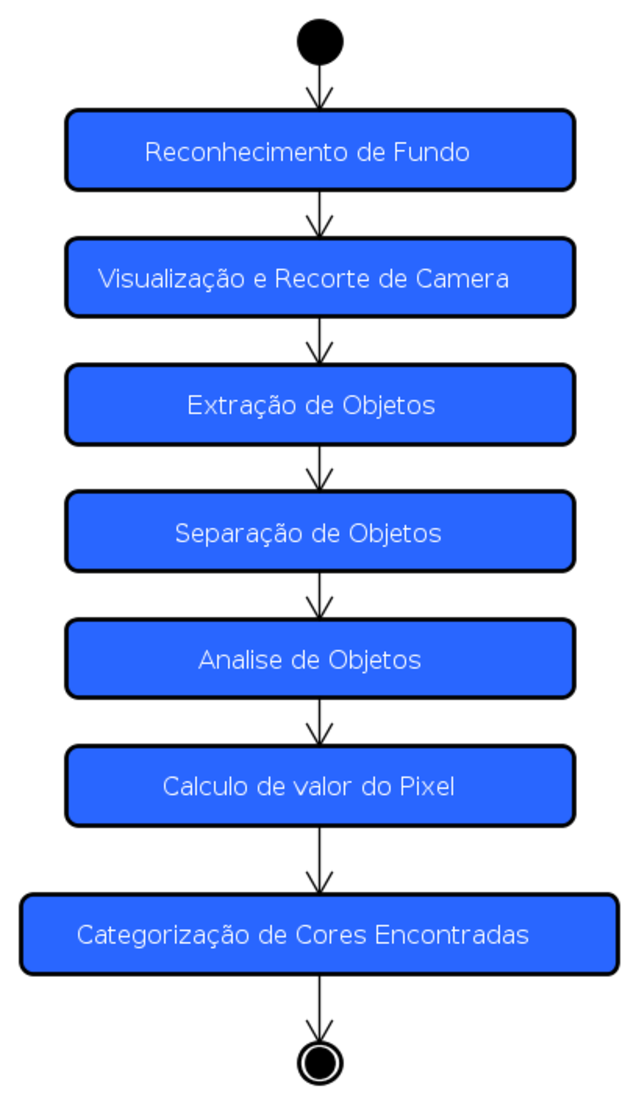
\includegraphics[width=0.45\textwidth]{FluxodoSistema.pdf}
			\caption{Diagrama de Fluxo}
			\label{fig:FlowCHart}
		\end{figure}			
Nas subseções à seguir serão detalhadas cada uma das etapas do processo de calibração automática.
		\subsection{1ª Etapa - Configuração de Câmera}
		

Para melhor desempenho do algoritmo de detecção de objetos, a imagem é recortada somente para o tamanho necessário. O recorte de imagem foi feito utilizando a função {\it setMouseCallback}, disponível pelo OpenCV, para possibilitar a interação do usuário na imagem utilizando o mouse, sua utilização é dada da seguinte maneira:
\begin{center}
\centering \textit{ cv::setMouseCallback(src\_window,mouseHandler,0);}
\end{center}
O primeiro parâmetro, \textbf{src\_windows}, indica a janela na qual a função recebera a interação. O segundo, \textbf{mouseHandler}, indica a função na qual esta implementada a interação. Já ultimo parâmetro, \textbf{0}, indica parâmetros opcionais.
Dentro da função \textbf{mouseHandler} são identificados os dois pontos da seleção, inicio e fim, além da utilização da função \textit{rectangle} para demarcar a seleção na tela. A função \textit{rectangle} foi utilizada da seguinte maneira:
\begin{center}
\centering \textit{ cv::rectangle(frameA, point1, point2, CV\_RGB(255, 0, 0), 2, 5, 0);}
\end{center}
A função recebe os parâmetros \textbf{frameA} indicando a imagem na qual será demarcada a área selecionada, depois o parâmetro \textbf{point1} que é o ponto inicial de seleção na imagem, \textbf{point2} que é o ponto final da seleção. \textbf{CV\_RGB(255, 0, 0)} que indica a cor da demarcação, \textbf{2} indicando a espessura da demarcação, \textbf{5} que significa o tipo de linha a ser utilizado na demarcação e \textbf{0} que é o numero de bits fracionários.

\begin{figure}[H]
			\centering
			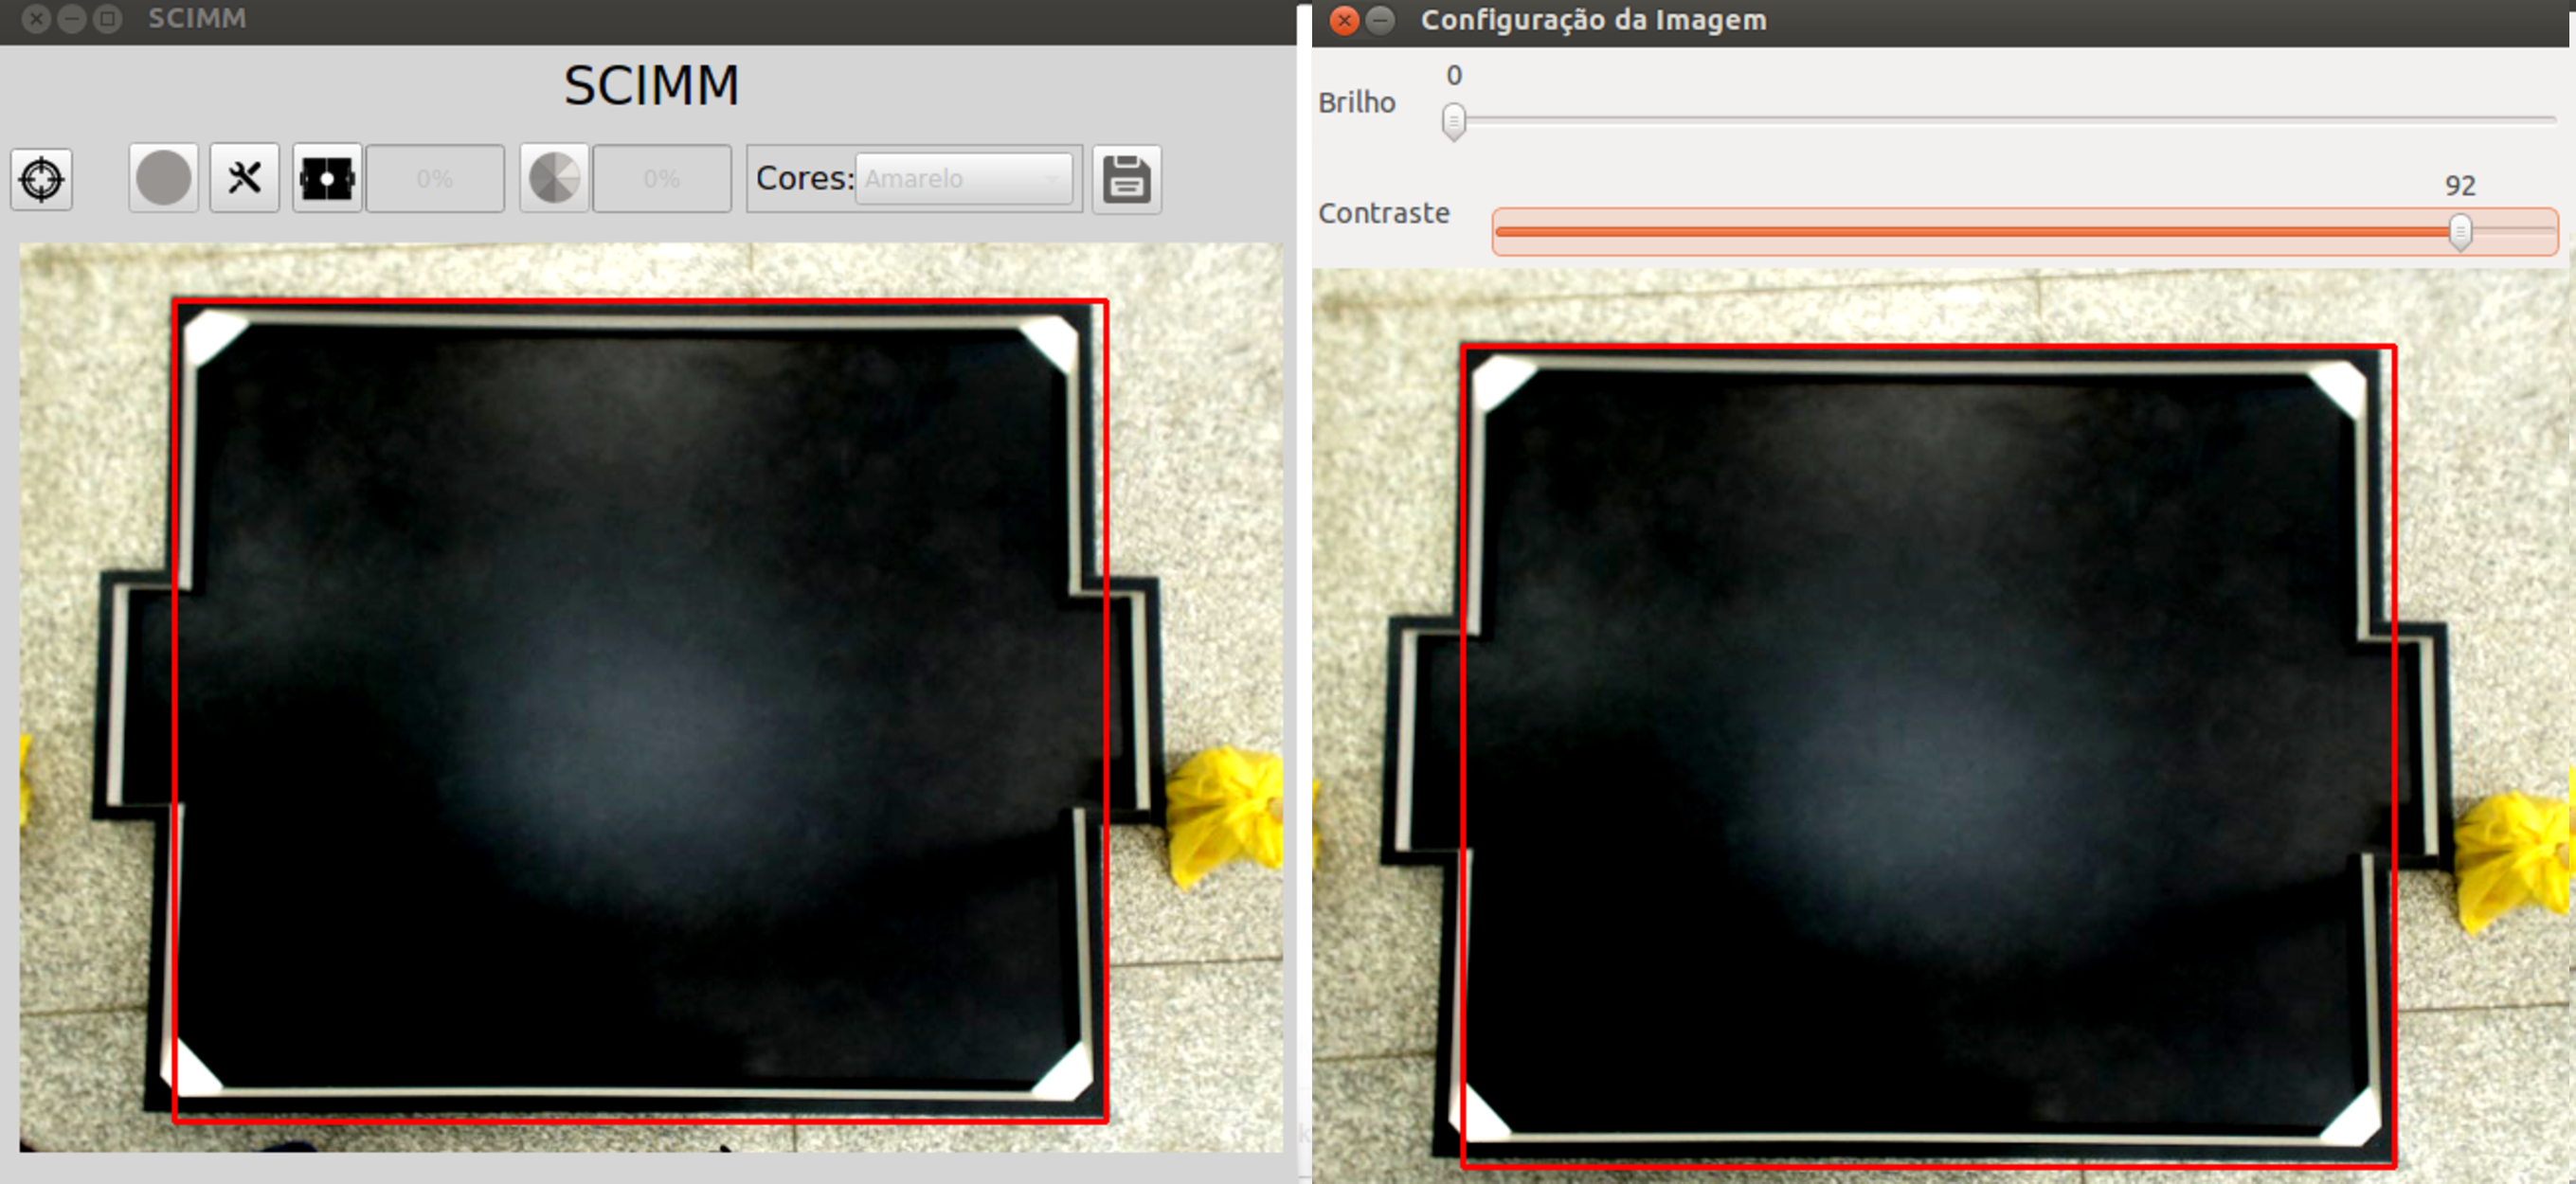
\includegraphics[width=0.8\textwidth]{passo1.pdf}
			\caption{ Configuração de Camera}
			\label{Configuracao}
		\end{figure}		


 Após confirmada a escolha, o tamanho da tela é salvo na variável nomeada \emph{tamanho}, usado durante todo o processo de calibração.
Além do recorte da imagem, nessa etapa também são configurados Brilho e Contraste, de forma que as cores no campo se tornem mais vívidos, e os objetos consequentemente mais nítidos, fazendo com que os processos de separação e detecção de objetos sejam mais precisos. A configuração de Brilho e Contraste utiliza o método \textit{convertTo} da biblioteca, que é utilizada para o melhoramento da imagem antes da detecção dos objetos. A utilização do método se deu por:
\begin{center}
\centering \textit{ frameA.convertTo(frameA, -1, contrast\_value / 50.0, brightness\_value -200)}
\end{center}
Esta função recebe quatro parâmetros. O primeiro \textbf{frameA} será o resultado da conversão. O segundo \textbf{-1} indica o tipo da matriz, ou numero de canais, da imagem a ser gerada, usa-se -1 quando se deseja que se use os valores semelhantes aos da imagem original\cite{OpenCV}. O terceiro \textbf{contrast\_value / 50.0} indica o valor de contraste, ou alpha, a ser usado para multiplicar os valores do pixel da imagem\cite{OpenCV} e por último \textbf{brightness\_value -200} que é o valor do brilho, ou beta, a ser adicionado à imagem. É importante ressaltar que a configuração de Brilho e Contraste é somente usada para a melhor precisão na detecção dos objetos, no momento da análise do pixel, a imagem não contêm alterações.\newline

	\subsection{2ª Etapa - Reconhecimento de Fundo}
	Um dos principais problemas que ocorrem na detecção de objetos é a confusão do fundo junto ao próprio objeto, fazendo com que o mesmo seja detectado com o contorno incorreto ou em outras vezes ignorando-o por ser considerado parte do fundo. Para eliminar este problema, foi utilizada a técnica de Subtração do fundo usando Mistura de Gaussianas, por meio do objeto \textit{createBackgroundSubtractorMOG2()} disponível na biblioteca OpenCV. Esta técnica utiliza um algoritmo de análise pixel a pixel, classificando-o com base na distribuição da gaussiana que o representa. Para separar o fundo do resto da imagem é levada em consideração que a gaussiana que representa o fundo tenha grande peso e baixa variância, isso significa que a mesma ocorre frequentemente e varie pouco com o tempo. O algoritmo atualiza o modelo de fundo a cada quadro da imagem, baseando-se na movimentação do objetos já contido na imagem ou na inserção ou remoção de objetos. O objeto criado pela biblioteca, por meio do método \textit{apply}, analisa quadro a quadro a imagem, e a compara com o fundo obtido e gera uma imagem chamada de \textbf{máscara}, contendo os objetos que não fazem parte do fundo, no exato momento de um quadro, com o passar dos quadros o objeto se torna parte do fundo. Uso do método:
\begin{center}
 \textit{pMOG2-$>$apply(frame, mask);}

\end{center}

No qual \textbf{frame} significa o quadro atual capturado pela câmera e \textbf{mask} a máscara gerada pela diferença da imagem atual com o modelo de fundo. 

\begin{figure}[H]
			\centering
			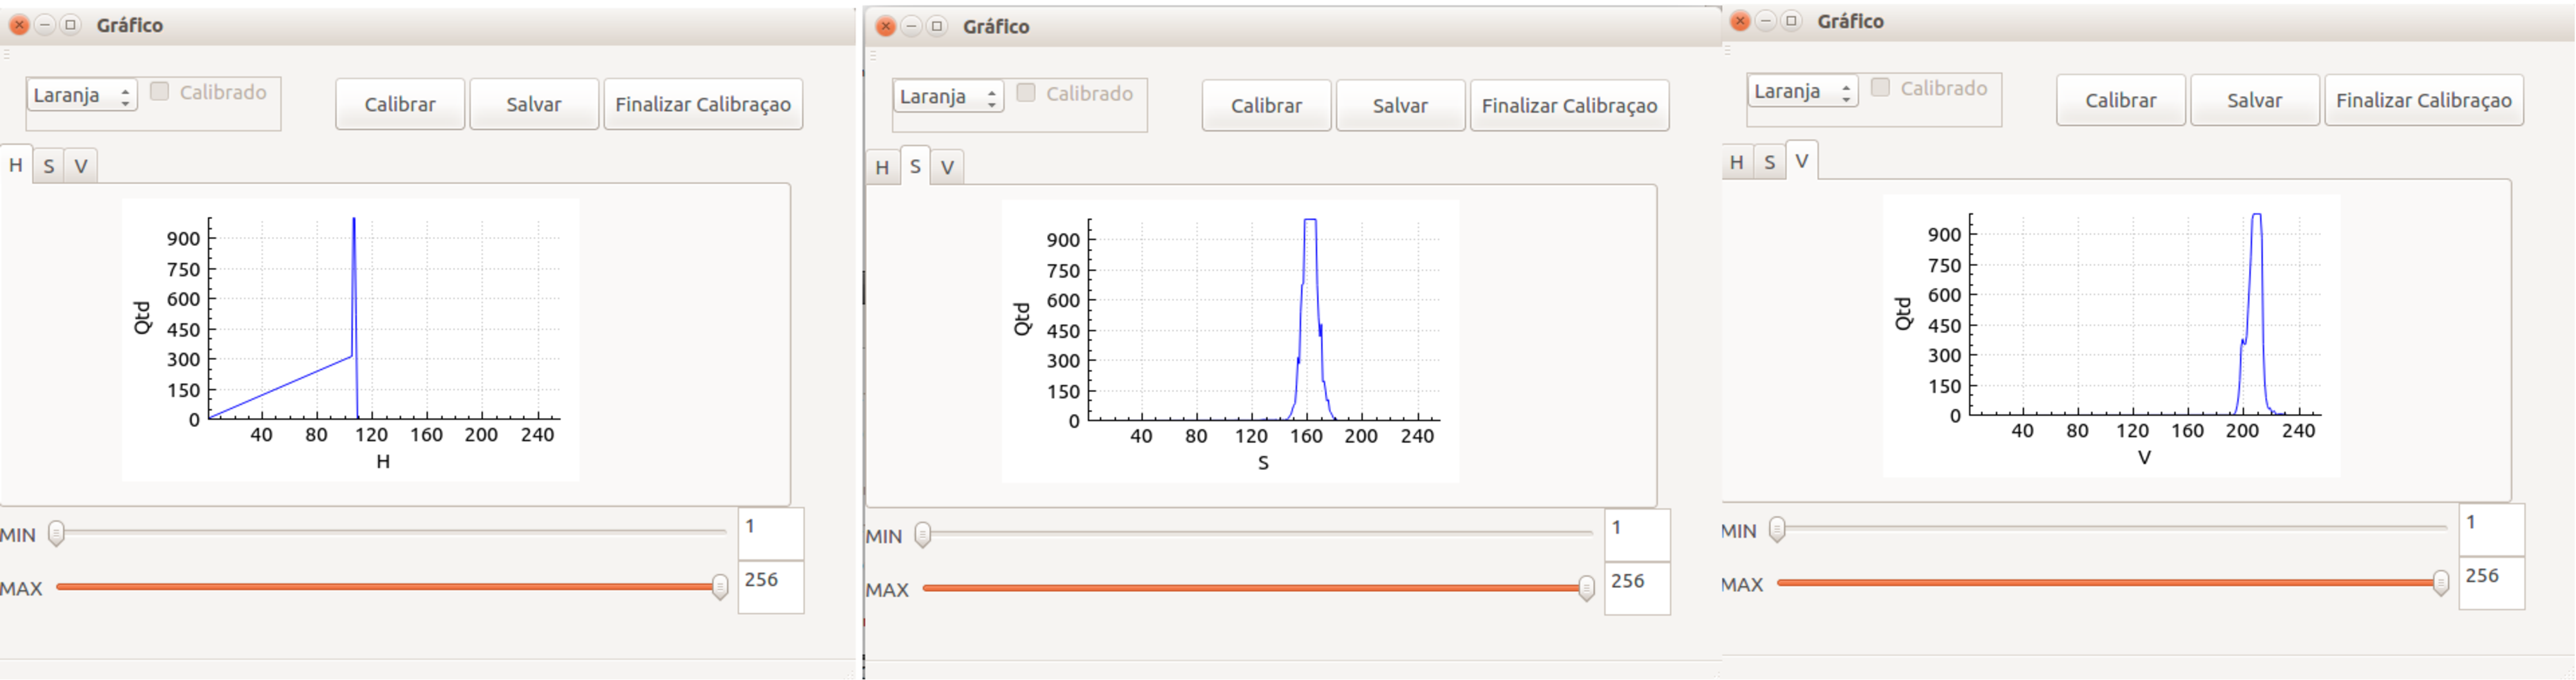
\includegraphics[width=0.45\textwidth]{passo2.pdf}
			\caption{Configuração de Camera}
			\label{Configuracao}
		\end{figure}		


Sabendo-se inicialmente que o modelo de fundo do objeto \textbf{pMOG2} está vazio, basta que ele seja executado algumas vezes para que o campo se torne o modelo de fundo. Nesse caso a máscara gerada pelo método não chega a ser utilizada.
	\subsection{3ª Etapa - Extração dos Objetos do Fundo}
	Como visto na 2ª etapa, o objeto \textbf{pMOG2} chamando o método \textit{apply} gera uma máscara de diferença da imagem atual para o modelo de fundo. Sendo assim para obtermos os objetos que virão a ser detectados, basta que o método \textit{apply} seja chamado um número de vezes suficientes para criar a máscara ao mesmo tempo que não altere o modelo de fundo.
	
\begin{figure}[H]
			\centering
			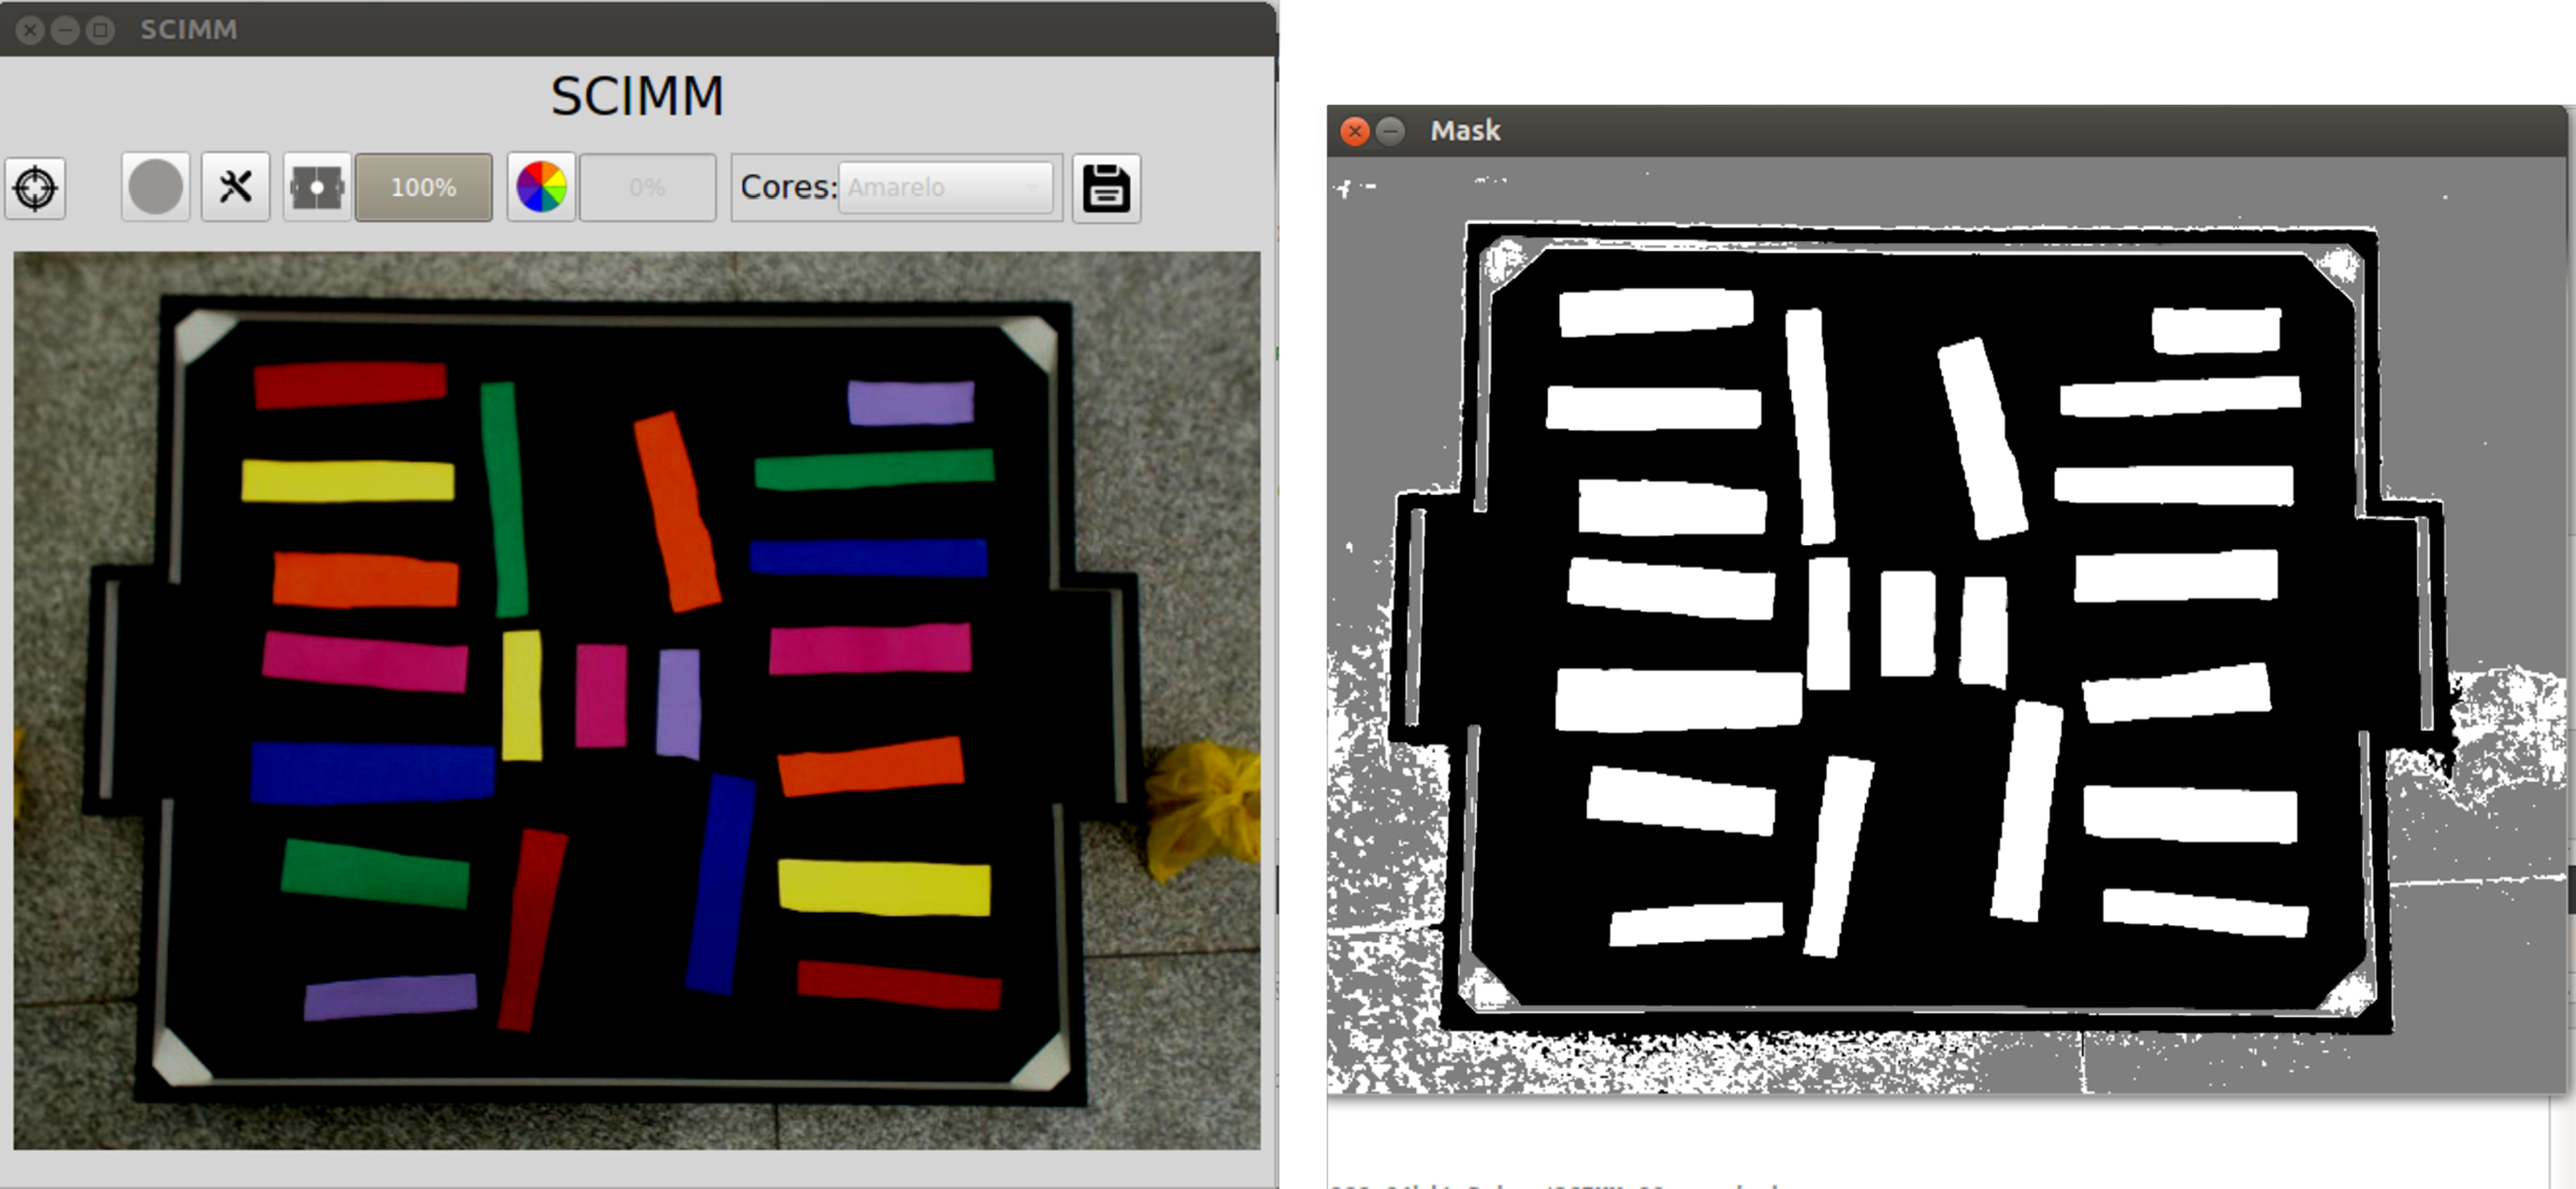
\includegraphics[width=0.8\textwidth]{passo3.pdf}
			\caption{Geração de Máscara}
			\label{Configuracao}
		\end{figure}		


\subsection{4ª Etapa - Detecção e validação de Objetos}
Para ser feita a detecção dos objetos é necessário que primeiro seja feita a detecção de bordas dos objetos. Como recurso para eliminação de ruídos e melhoria da imagem, antes de ser executada a detecção, utiliza-se o desfoque na imagem. O algoritmo de detecção de bordas utilizado no desenvolvimento foi o algoritmo de Canny, descrito na Seção 2.2.2, que é implementado pela biblioteca OpenCV, e foi utilizado neste trabalho como segue:
\begin{center}
\centering \textit{  Canny(src\_gray, canny\_output, limiar, limiar * 3, 3);}
\end{center}

O algoritmo de Canny utiliza por padrão imagem em escalas de cinza, sendo assim \textbf{src\_gray} é a imagem original transformada para escala de cinza, na qual o algoritmo será aplicado. \textbf{canny\_output} será a imagem de saída da função.
\textbf{limiar} e \textbf{limiar*3} são os limites mínimos e máximos, respectivamente, para considerar uma borda. \textbf{3} é o valor de apertura ou kernel, sendo o valor 3 é utilizado como padrão.

Após o uso do algoritmo de Canny para detecção de bordas, é necessário então fazer uso da função \textit{findContours}, nativa no OpenCV que utiliza do algoritmo {\it border following} para fazer a detecção de objetos aqui chamados de contornos.
\begin{center}
\centering \textit{ findContours(canny\_output, contours, hierarchy, CV\_RETR\_EXTERNAL, CV\_CHAIN\_APPROX\_SIMPLE, Point(0, 0))}
\end{center}

O primeiro parâmetro, \textbf{canny\_output}, é a imagem que o algoritmo de Canny gerou com as bordas encontradas, e que será utilizada pelo método \textit{findContours} para detectar os contornos. \textbf{contours} é o parâmetro que armazenará os contornos encontrados, no qual cada contorno é armazenado como sendo um vetor de pontos. Na variável \textbf{hierarchy} será salvo um vetor de informações sobre a topologia da imagem, e terá como total de elementos o mesmo número que o total de contornos encontrados. O quarto parâmetro, \textbf{CV\_RETR\_EXTERNAL} indica o modo de obtenção de contornos, nesse caso \textbf{CV\_RETR\_EXTERNAL} indica que o método só obterá os contornos exteriores. \textbf{CV\_CHAIN\_APPROX\_SIMPLE} designa o método de aproximação de contornos utilizado, o método utilizado comprime segmentos horizontais, verticais e diagonais os deixando apenas com seus pontos finais. O último parâmetro, \textbf{Point(0, 0)}, indica o valor a ser usado para deslocar a imagem ao encontrar os objetos, neste caso esse valor é 0 para Y e 0 para X, pois não haverá deslocamento \cite{OpenCV}. 

Uma vez obtidos os contornos é necessários que se faça a eliminação de vértices dos polígonos encontrados nos objetos, deixando o objeto mais preciso. Isso é necessário para deixar a forma encontrada mais semelhante com a forma original do objeto. Para este ajuste foi usado o método \textit{approxPolyDP}, já implementado dentro na biblioteca OpenCV. Este método foi aplicado em cada um dos contornos encontrados, e foi utilizado como mostrado a seguir:
\begin{center}
\centering \textit{    approxPolyDP(Mat(contours[i]), contours\_poly[i], 3, true)}
\end{center}

O método inicia recebendo como parâmetro \textbf{Mat(contours[i])}, que é a criação de uma nova imagem, somente com aquele único objeto que esta sendo analisado. A seguir é informado no segundo parâmetro a variável de destino \textbf{contours\_poly[i]}, na qual será armazenado o objeto com a eliminação dos vértices. O terceiro parâmetro indica o valor do \textit{epilson}, usado o valor \textbf{3}, a distância máxima entre a curva original para sua aproximação\cite{OpenCV}. O último parâmetro indica se a curva aproximada será fechada ou não, foi usado o valor \textbf{true}.

Por último os objetos possuem sua borda ignorada, calculando o tamanho interior deles para que, por ventura, não hajam pixeis de cor preta ou escurecidos devido a proximidade da borda.
 
 \subsection{5ª Etapa - Classificação do Pixel}

 
 
 Para ser feita a classificação do pixel é necessário que se faça primeiramente a conversão da imagem obtida pela câmera. A imagem proveniente da câmera está no modelo de cores RGB, e será convertida para o modelo HSV, pois este lida melhor com diferentes tonalidades.
  
 A biblioteca OpenCV converte o espaço de cor usando a função \textit{cvtColor}, que recebe como parâmetro a imagem original, e uma imagem vazia com memória alocada, onde será salva a imagem após a conversão, além do parâmetro do tipo de conversão. Exemplo do uso do método:
\begin{center}
\centering \textit{cvtColor(frame, HSV, CV\_RGB2HSV);}
\end{center}

Após a conversão, é necessário ser feita uma análise dos objetos encontrados. Para cada objeto serão analisados todos os seus pixeis separadamente, e categorizados de acordo com o intervalo de valores de H representados na Tabela \ref{tab:categorias}. Esta tabela foi gerada, durante a pesquisa e implementação do sistema SCIMM, a partir das observações da representação do modelo de cor HSV do OpenCV, que difere da teoria das cores.

\begin{table}[H]
\centering
\begin{tabular}{r|r}
Cor & Intervalo de H \\ % Note a separação de col. e a quebra de linhas
\hline                               % para uma linha horizontal
Laranja & de 0 à 20 \\
\hline 
Amarelo & de 21 à 30\\
\hline 
Verde & de 61 à 90 \\
\hline 
Azul& de 91 à 120 \\
\hline 
Roxo & de 125 à 160 \\
\hline 
Rosa & de 161 à 168 \\
\hline 
Vermelha & de 169 à 180 \\
\hline 
\end{tabular}
\caption{Intervalo de Valores de Cores - HSV do OpenCV}
\label{tab:categorias}
\end{table}

Durante o desenvolvimento foi observador que, em sua maioria, as cores necessitavam de um valor (S,V) pré estabelecidos. Para as cores Laranja, Azul, Rosa e Vermelho foi pré estabelecido o valor (100,100). A cor Amarelo usa a pré definição (50,50). A cor Verde é a única que possui os valores pré definidos diferenciados um do outro, tendo 30 para S e 50 para V, ou seja (30,50). Já a cor Roxo, (30,30), possui tanto para S quanto para V o valor 30.

  \subsection{6ª Etapa - Gerar Arquivo de Cores}
  Assim que todas as cores já estiverem sido assimiladas e a calibração finalizada, gera-se um arquivo chamado \textbf{cores.arff}, contendo 14 linhas. Sabendo que o sistema calibra 7 cores, o arquivo gerado contem duas linhas para cada cor, sendo a primeira com o valores mínimos de H, S e V e a segunda com o valores máximos.

\section{Considerações Finais}


 O projeto desenvolvido conta com funcionalidades bem dividas, e cada classe exerce somente um único papel. Com a utilização da biblioteca OpenCV, conseguiu-se atender todos os objetivos relacionados ao processamento digital de imagens necessários para o desenvolvimento do sistema proposto.

 O sistema consiste em um único módulo, em cinco partes principais: (1) detecção de bordas da imagem, (2) identificação dos objetos por meio das bordas encontradas, (3) análise de pixeis nos objetos, (4) categorização do HSV do pixel e (5) criação do arquivo com os valores mínimos e máximos para cada cor. É importante destacar que todos os processos do sistema acontecem de forma automática.
  
 